\documentclass[../../main.tex]{subfiles}

\graphicspath{{../../image/}{../../figure/}}

\begin{document}

\subsection{实战中的 GAN 训练}\label{subsection:ch17-实战GAN训练}

尽管 GAN 可以产生高质量的结果，但由于对抗学习的特点，其并不容易训练成功（见\cref{exercise:ch17-02}）。此外，与标准的损失函数最小化不同，由于目标函数的值在训练过程中可能上升也可能下降，因此并没有一个明确的进展指标。

\begin{definition}[模式崩溃]\label{definition:ch17-模式崩溃}
在 GAN 的训练过程中，生成器网络的权重可能发生适应性调整，导致所有潜变量样本 $z$ 都被映射到有效输出的一个子集上；在极端情况下，输出可能只对应一个或少数几个输出值 $x$，判别器网络随后将这些实例的值设置为 $0.5$ 并停止训练。称这一现象为\textbf{模式崩溃}（mode collapse）。
\end{definition}

% SUPPLEMENT: parent=definition:ch17-模式崩溃; kind=motivation; location=紧随其后的 remark（重构新增）
\begin{remark}（重构新增）
模式崩溃的根源在于生成器的目标只要求“骗过判别器”，而不要求“覆盖数据分布”：若 $p_g$ 把全部质量堆在 $p_{\mathrm{data}}$ 的某个峰上，判别器在该峰附近无法区分真假，生成器的损失就已经很小，尽管其余的模式完全没有被生成。用\cref{proposition:ch17-最优判别器}的语言说，此时 $p_g$ 与 $p_{\mathrm{data}}$ 的 Jensen-Shannon 散度并不为零，但在有限容量的参数化下，生成器可以停在一个使判别器“局部失效”的驻点上。

条件方面：模式崩溃是优化与参数化的联合现象，而不是目标函数在无限容量下的性质——\cref{proposition:ch17-最优判别器}表明，若生成器能在全部概率分布上优化，最优解恰是 $p_g=p_{\mathrm{data}}$，不会崩溃。此外，判别器输出被置为 $0.5$ 意味着它对真实样本与合成样本给出相同的概率，这既可能来自 $p_g$ 与 $p_{\mathrm{data}}$ 的局部重合，也可能来自判别器自身的容量不足，两者在训练中很难区分，这也是 GAN 缺乏可靠进展指标的一个具体表现。
\end{remark}

\begin{example}[ 手写数字生成中的模式崩溃]\label{example:ch17-模式崩溃}
一个用于生成手写数字的 GAN 可能学会只生成数字“3”的实例，而判别器网络无法将这些实例与真正的数字“3”的实例区分开来，它没能认识到生成器网络并没有生成所有可能的数字。
\end{example}

通过\cref{figure:ch17-一维判别器}，我们可以更深入地理解训练 GAN 的困难。该图显示了一个简单的一维数据空间 $x$，其中样本 $\{x_n\}$ 来自固定但未知的数据分布 $p_{\mathrm{data}}(x)$。该图还显示了初始生成分布 $p_g(x)$ 以及从该分布中抽取的样本。因为数据分布和生成分布之间差异显著，最优的判别器函数 $d(x)$ 很容易学习，其函数值下降态势急剧，在真实样本或合成样本的邻近区域梯度几乎为零。考虑 GAN 损失函数［\eqref{align:ch17-GAN损失}］中的第二项，由于在生成样本跨越的区域内 $d(g(z,w),\phi)$ 值等于零，生成器网络参数 $w$ 的微小变化在判别器网络的输出上将产生很小的变化，因此梯度较小，导致学习进程缓慢。

\begin{figure}[htbp]
  \centering
  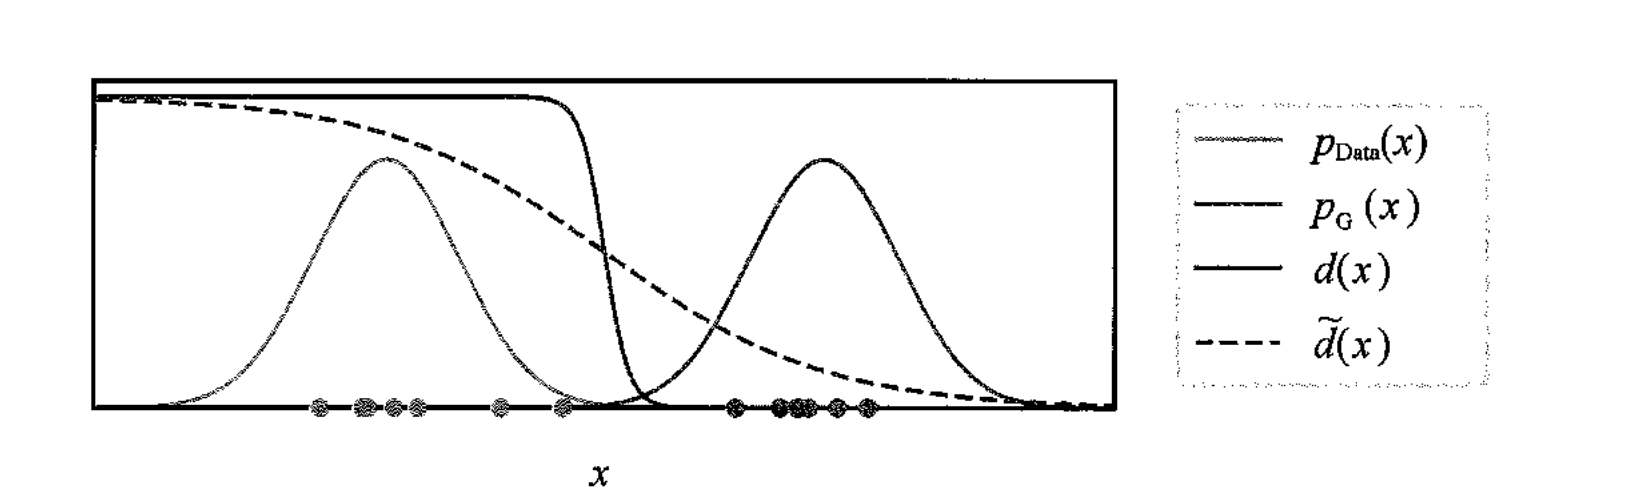
\includegraphics[width=0.82\textwidth]{ch17-fig487-one-d.png}
  \caption{为了从概念上说明为什么训练 GAN 可能会有难度，这里展示了一个简单的一维数据空间 $x$，其中有固定但未知的数据分布 $p_{\mathrm{data}}(x)$ 和初始生成分布 $p_g(x)$。最优的判别函数 $d(x)$ 在训练或合成数据点附近几乎没有梯度，使学习变得非常缓慢。判别函数的平滑版本 $\tilde{d}(x)$ 可以使学习变得更快}
  \label{figure:ch17-一维判别器}
\end{figure}

这个问题可以通过使用判别器函数的平滑版本 $\tilde{d}(x)$ 来解决（见\cref{figure:ch17-一维判别器}），从而为生成器网络提供更强的梯度以驱动训练。最小二乘 GAN（least-squares GAN, Mao et al., 2016）通过修改判别器网络输出一个实值而不是取值范围为 $0\sim1$ 的概率，并用平方和损失函数替换交叉熵损失函数来实现平滑。另一种称为\textbf{实例噪声}（instance noise）（Sønderby et al., 2016）的方法则向真实样本和合成样本中添加 Gauss 噪声，这同样能使判别器函数更加平滑。

为了改进 GAN 的训练，研究者们提出了许多对损失函数和训练过程的修改方案（Mescheder, Geiger, and Nowozin, 2018）。其中常见的一个建议是将原始损失函数中的生成器网络
\begin{align}
-\frac{1}{N_{\mathrm{synth}}}\sum_{n\in\mathrm{synth}}\ln\big(1-d(g(z_n,w),\phi)\big)
\label{align:ch17-生成器原始目标}
\end{align}
替换为
\begin{align}
\frac{1}{N_{\mathrm{synth}}}\sum_{n\in\mathrm{synth}}\ln d(g(z_n,w),\phi).
\label{align:ch17-生成器替代目标}
\end{align}

\eqref{align:ch17-生成器原始目标}所示的第一种形式最小化了图像为假的概率，\eqref{align:ch17-生成器替代目标}所示的第二种形式则最大化了图像为真的概率。这两种形式的不同属性可以通过\cref{figure:ch17-损失曲线}来加以理解。当生成分布 $p_g(x)$ 与数据分布 $p_{\mathrm{data}}(x)$ 完全不重叠时，$d(g(z,w))$ 接近于零，因此第一种形式具有非常小的梯度，而第二种形式具有较大的梯度，从而能加快训练速度。

\begin{figure}[htbp]
  \centering
  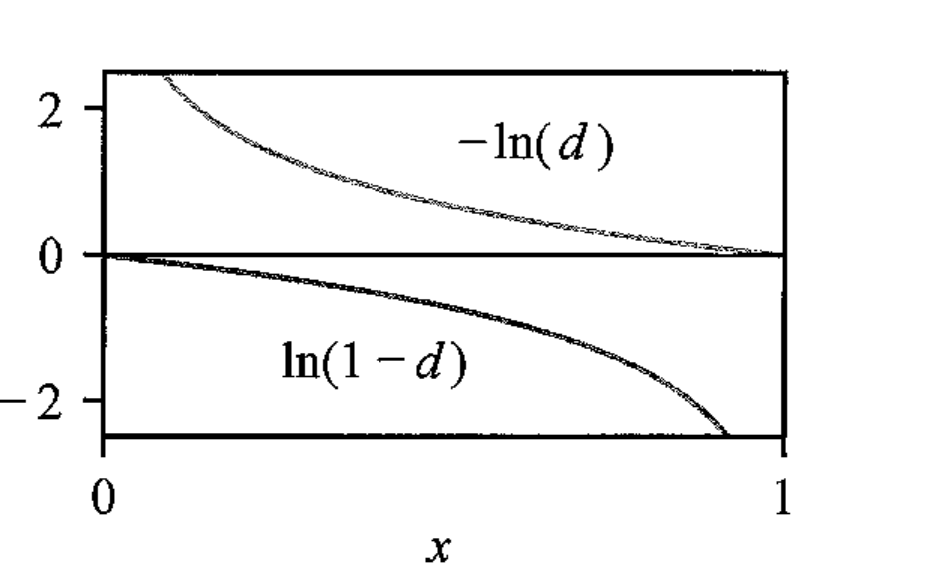
\includegraphics[width=0.62\textwidth]{ch17-fig487-loss-curves.png}
  \caption{$-\ln(d)$ 和 $\ln(1-d)$ 的图像表明，在 $d=0$ 和 $d=1$ 附近，梯度的表现存在非常大的差异}
  \label{figure:ch17-损失曲线}
\end{figure}

为确保生成分布 $p_g(x)$ 向数据分布 $p_{\mathrm{data}}(x)$ 靠拢，更直接的方法是修改误差标准，以反映这两个分布在数据空间中的距离。这可以使用\textbf{Wasserstein 距离}（也称推土机距离）来衡量。设想生成分布 $p_g(x)$ 是一堆土，我们需要分批运输这堆土以构建数据分布 $p_{\mathrm{data}}(x)$。Wasserstein 距离就是移动的土壤总量和平均移动距离的积。在重排这堆土以构建 $p_{\mathrm{data}}(x)$ 的许多方式中，能产生最小平均移动距离的方式被用于定义度量。

\begin{definition}[Wasserstein 距离]\label{definition:ch17-Wasserstein距离}
设 $p$ 与 $q$ 是 $\mathbb{R}^D$ 上的概率分布，$\Pi(p,q)$ 表示边缘分布分别为 $p$ 与 $q$ 的全部联合分布的集合。称
\begin{align*}
W(p,q)=\inf_{\gamma\in\Pi(p,q)}\mathbb{E}_{(x,y)\sim\gamma}\big[\|x-y\|\big]
\end{align*}
为 $p$ 与 $q$ 之间的\textbf{Wasserstein 距离}（Wasserstein distance），也称\textbf{推土机距离}（earth mover distance）；$\gamma$ 称为从 $p$ 到 $q$ 的一个\textbf{传输方案}（transport plan）。
\end{definition}

% SUPPLEMENT: parent=definition:ch17-Wasserstein距离; kind=motivation; location=紧随其后的 remark（重构新增）
\begin{remark}（重构新增）
定义中的 $\gamma$ 就是“运输方案”：$\gamma(A\times B)$ 表示从区域 $A$ 运往区域 $B$ 的土壤量，边缘条件 $\gamma(A\times\mathbb{R}^D)=p(A)$、$\gamma(\mathbb{R}^D\times B)=q(B)$ 保证出发点与目的地的土量分别与 $p$、$q$ 相符。由于总质量已被归一化为 $1$，“移动的土壤总量与平均移动距离的积”就是平均移动距离本身，即 $\mathbb{E}_\gamma[\|x-y\|]$；取 $\inf$ 对应原书所说的“能产生最小平均移动距离的方式”。

与 Jensen-Shannon 散度相比，Wasserstein 距离的最大好处是它在两个分布的支撑集互不相交时仍然提供有意义的数值：若 $p$ 与 $q$ 的支撑集之间的距离为 $d>0$，则 $W(p,q)\geqslant d>0$，而 $\operatorname{JSD}(p\|q)$ 恒等于 $\ln 4$（与两个支撑集的距离无关），其梯度为零。这解释了为什么\cref{proposition:ch17-最优判别器}意义下的 GAN 在训练初期（$p_g$ 与 $p_{\mathrm{data}}$ 几乎不重叠）没有可用的梯度信号，而以 $W$ 为目标的模型不会遇到这一问题。

条件方面：$\Pi(p,q)$ 非空（乘积分布即为一个传输方案），故 $\inf$ 有定义；$\|\cdot\|$ 取哪个范数会影响数值但不影响“$W(p,q)=0\iff p=q$”这一性质。此外 $W$ 是对称的、满足三角不等式，因此是真正的度量，而 $\operatorname{JSD}^{1/2}$ 才是度量、$\operatorname{JSD}$ 本身不是。
\end{remark}

在实践中，这并不能直接实现，需要通过使用一个具有实值输出的判别器网络来近似，然后通过权重裁剪限制判别器函数关于 $x$ 的梯度 $\nabla_x d(x,\phi)$，从而产生了 Wasserstein GAN（Arjovsky, Chintala, and Bottou, 2017）。

另一种改进的方法是对梯度引入惩罚，从而产生了梯度惩罚 Wasserstein GAN（Gulrajani et al., 2017），其损失函数由下式给出：
\begin{align}
E_{\mathrm{WGAN}\text{-}\mathrm{GP}}(w,\phi)={}&-\frac{1}{N_{\mathrm{real}}}\sum_{n\in\mathrm{real}}\Big[\ln d(x_n,\phi)-\eta\big(\|\nabla_{x_n}d(x_n,\phi)\|^{2}-1\big)^{2}\Big]_{+}\nonumber\\
&+\frac{1}{N_{\mathrm{synth}}}\sum_{n\in\mathrm{synth}}\ln d\big(g(z_n,w,\phi)\big),
\label{align:ch17-WGAN-GP}
\end{align}
其中的 $\eta$ 控制了惩罚项的相对重要性。

\begin{remark}（重构新增）
\eqref{align:ch17-WGAN-GP}的结构可以逐项读出：第一项对真实样本要求 $\ln d(x_n,\phi)$ 尽量大，同时用 $\big(\|\nabla_{x_n}d\|^{2}-1\big)^{2}$ 把判别器在真实样本处的梯度范数拉向 $1$；第二项对合成样本要求 $\ln d$ 尽量小；外层的 $[\cdot]_+$ 是 hinge（只惩罚超过零的部分），使损失在达到间隔后不再继续下降。

需要指出原文的一处技术细节：标准的梯度惩罚项写作 $\big(\|\nabla_{\hat{x}}d(\hat{x},\phi)\|-1\big)^2$，其中 $\hat{x}$ 在真实样本与合成样本之间随机插值；\eqref{align:ch17-WGAN-GP}把范数写成了平方 $\|\cdot\|^{2}$，并把取样点取在真实样本 $x_n$ 上。二者都是对“判别器应为 1-Lipschitz”这一约束的可计算松弛，只是松弛的位置不同：前者约束梯度范数等于 $1$，后者约束梯度范数的平方等于 $1$，由于 $\|\nabla d\|\geqslant0$，两式的零点都恰是 $\|\nabla d\|=1$，故在最优点处二者一致。此外，$\eta$ 在原文中控制惩罚项的权重，其作用与 Lagrange 乘子相同：$\eta$ 越大，约束越被强制满足，但训练也越不稳定。
\end{remark}

\begin{proposition}[Kantorovich-Rubinstein 对偶]\label{proposition:ch17-KR对偶}
设 $\mathcal{X}$ 是 $\mathbb{R}^D$ 中的紧集，$\|\cdot\|$ 是 $\mathbb{R}^D$ 上的范数，$p,q$ 是 $\mathcal{X}$ 上的概率分布。则
\begin{align}
W(p,q)=\sup_{f\in\operatorname{Lip}_1}\Big\{\mathbb{E}_{x\sim p}\big[f(x)\big]-\mathbb{E}_{y\sim q}\big[f(y)\big]\Big\},
\label{align:ch17-KR对偶}
\end{align}
其中 $\operatorname{Lip}_1$ 表示 $\mathcal{X}$ 上全部满足 $|f(x)-f(y)|\leqslant\|x-y\|$ 的实值函数（称为 1-Lipschitz 函数）的集合。
\end{proposition}

\begin{proof}（重构新增）
先证“$\geqslant$”。设 $f$ 是 1-Lipschitz 函数，$\gamma\in\Pi(p,q)$ 是任一传输方案。则
\begin{align*}
\mathbb{E}_{x\sim p}\big[f(x)\big]-\mathbb{E}_{y\sim q}\big[f(y)\big]
&=\int_{\mathcal{X}\times\mathcal{X}}\big(f(x)-f(y)\big)\mathrm{d}\gamma(x,y)\\
&\leqslant\int_{\mathcal{X}\times\mathcal{X}}\big|f(x)-f(y)\big|\,\mathrm{d}\gamma(x,y)
\leqslant\int_{\mathcal{X}\times\mathcal{X}}\|x-y\|\,\mathrm{d}\gamma(x,y),
\end{align*}
第一个等号用到 $\gamma$ 的边缘条件。对 $\gamma$ 取下确界得 $\mathbb{E}_p[f]-\mathbb{E}_q[f]\leqslant W(p,q)$，再对 $f$ 取上确界即得 $\sup\leqslant W(p,q)$。

再证“$\leqslant$”。先设 $\mathcal{X}$ 是有限点集 $\{x_1,\cdots,x_m\}$，记 $p_i=p(\{x_i\})$、$q_j=q(\{x_j\})$、$C_{ij}=\|x_i-x_j\|$。此时 $W(p,q)$ 是线性规划
\begin{align*}
\min\Big\{\sum_{i,j}\gamma_{ij}C_{ij}:\ \gamma_{ij}\geqslant0,\ \sum_{j}\gamma_{ij}=p_i,\ \sum_{i}\gamma_{ij}=q_j\Big\}
\end{align*}
的最优值。由线性规划对偶定理，它等于对偶问题
\begin{align*}
\max\Big\{\sum_{i}a_ip_i+\sum_{j}b_jq_j:\ a_i+b_j\leqslant C_{ij}\ \text{对一切}\ i,j\Big\}
\end{align*}
的最优值。设 $(a,b)$ 是对偶可行解，令 $f_i=\min_j\big(C_{ij}-b_j\big)$。由三角不等式，对任意 $i,k$ 及取得最小值的 $j^*$ 有
\begin{align*}
f_i-f_k\leqslant\big(C_{ij^*}-b_{j^*}\big)-\big(C_{kj^*}-b_{j^*}\big)=C_{ij^*}-C_{kj^*}\leqslant C_{ik},
\end{align*}
交换 $i,k$ 可得反向不等式，故 $f$ 是 1-Lipschitz 的；又 $f_j\leqslant C_{jj}-b_j=-b_j$，故
\begin{align*}
\sum_{i}a_ip_i+\sum_{j}b_jq_j\leqslant\sum_{i}f_ip_i-\sum_{j}f_jq_j=\mathbb{E}_{p}[f]-\mathbb{E}_{q}[f]\leqslant\sup_{g\in\operatorname{Lip}_1}\Big\{\mathbb{E}_{p}[g]-\mathbb{E}_{q}[g]\Big\}.
\end{align*}
于是 $W(p,q)\leqslant\sup$，与前一方向合并即得\eqref{align:ch17-KR对偶}。

对一般的紧集 $\mathcal{X}$，上述论证可以这样移植。取 $\mathcal{X}$ 的有限 $\varepsilon$-网 $\{x_1,\cdots,x_m\}$ 与投影 $\pi:\mathcal{X}\to\{x_1,\cdots,x_m\}$，使 $\|x-\pi(x)\|\leqslant\varepsilon$ 对一切 $x$ 成立，并记 $p^{\varepsilon},q^{\varepsilon}$ 为 $p,q$ 在 $\pi$ 下的像。任取 $(p,q)$ 的传输方案 $\gamma$，其像 $(\pi(x),\pi(y))_{\sharp}\gamma$ 是 $(p^{\varepsilon},q^{\varepsilon})$ 的传输方案，且 $\|x-y\|\leqslant\|\pi(x)-\pi(y)\|+2\varepsilon$，故 $W(p,q)\leqslant W(p^{\varepsilon},q^{\varepsilon})+2\varepsilon$。另一方面，$\mathcal{X}$ 上的 1-Lipschitz 函数限制在网上仍为 1-Lipschitz，且 $|f(x)-f(\pi(x))|\leqslant\varepsilon$，故 $\mathbb{E}_{p^{\varepsilon}}[f]-\mathbb{E}_{q^{\varepsilon}}[f]\leqslant\mathbb{E}_{p}[f]-\mathbb{E}_{q}[f]+2\varepsilon$。把离散情形的结论用于 $p^{\varepsilon},q^{\varepsilon}$ 并令 $\varepsilon\to0$，即得 $W(p,q)\leqslant\sup$。这一论证的一般形式就是 Kantorovich-Rubinstein 定理，它也可由 Hahn-Banach 定理在 $C(\mathcal{X})$ 上直接导出。
\end{proof}

% SUPPLEMENT: parent=proposition:ch17-KR对偶; kind=motivation; location=紧随其后的 remark（重构新增）
\begin{remark}（重构新增）
\eqref{align:ch17-KR对偶}是 Wasserstein GAN 的全部理论依据：它把一个“在联合分布上求下确界”的传输问题换成了“在一个函数类上求上确界”的问题，而后者可以直接用神经网络参数化——取 $f=d(\cdot,\phi)$，就得到
\begin{align*}
\max_{\phi}\Big\{\mathbb{E}_{x\sim p_{\mathrm{data}}}\big[d(x,\phi)\big]-\mathbb{E}_{z\sim p(z)}\big[d(g(z,w),\phi)\big]\Big\},
\end{align*}
这正是 WGAN 中判别器（此时称 critic，因为它输出实值而不是概率）要最大化的量；生成器则最小化同一量。原书所说的“权重裁剪”就是对 $\operatorname{Lip}_1$ 这一约束的粗糙实现：把每个权重的绝对值截断在 $[-c,c]$ 内，可以使网络所表示的函数具有与 $c$ 和层数有关的 Lipschitz 常数。权重裁剪把约束变成硬投影，容易造成梯度消失或爆炸；\eqref{align:ch17-WGAN-GP}的梯度惩罚则是把约束写成软惩罚，因而更稳定。

条件方面：命题要求 $\mathcal{X}$ 紧、$p,q$ 是 Borel 概率测度，这保证 $\Pi(p,q)$ 弱紧、$\inf$ 可达；若 $\mathcal{X}$ 非紧，结论对“有界 1-Lipschitz 函数”仍成立，但上确界可能不可达。还要注意\eqref{align:ch17-KR对偶}中的 $f$ 不带符号约束，因此 $\sup$ 一定非负（取 $f\equiv0$ 得 $0$），这与 $W\geqslant0$ 相符。
\end{remark}

\end{document}
